\documentclass[11pt]{article}
\usepackage[margin = 1in]{geometry}
\usepackage{amsmath}
\usepackage{amssymb}
\usepackage{amsthm} % for proof environment
\usepackage{enumitem}
\usepackage{graphicx}
\usepackage{indentfirst}
\usepackage{caption}
\usepackage{lscape}
\usepackage{multirow}
\usepackage{array}
\usepackage{setspace}
\setlist{nolistsep}
\usepackage[round]{natbib}
\usepackage{accents}
\usepackage{caption}
\usepackage{subcaption}
\usepackage{xcolor}
\usepackage{setspace}
\onehalfspacing
\interfootnotelinepenalty = 10000 % prevent the breaking of footnotes

\newtheorem{proposition}{Proposition}
\newtheorem{lemma}{Lemma}

% Front matter
\title{Optimal Taxation with Heterogeneous Rates of Return}
\author{
    Nicholas Hoffman\\
    \and 
    Ali Shourideh\\
}
\date{\today}

\begin{document}
\maketitle

\begin{abstract}
    We study optimal nonlinear taxation of capital income in an environment in which agents are heterogeneous in the returns that they earn on investments. Agents in our model can borrow and lend to one another at a constant rate, and invest in private entrepreneurial technology with idiosyncratic returns. In a two-period setting, we demonstrate that income streams from both saving and investing should be taxed at positive, but differential, rates. The optimal wedges on both assets are U-shaped over the space of possible returns, and shaped in part by the \textit{societal} marginal product of capital for an entrepreneur of a given type at the optimum. In the infinite-horizon extension, we derive a recursive form for the component planning problem.
\end{abstract}

\section{Introduction} \label{sec:intro}

The fact that capital income is the proximate force in shaping the wealth distribution in advanced economies is well established---see, for instance, \cite{benhabib2011distribution} or \cite{benhabib2019wealth}. The fortunes of those on the top rung of the economic ladder are primarily composed of high-risk, high-return assets, such as ownership of businesses and shares of stock. Those who hold these fortunes are largely entrepreneurs, investors, and business owners---talented individuals who face a range of rates of return in accumulating their wealth. Given these forces behind the wealth distribution, however, it is less clear what sort of tax and transfer system is optimal to both satisfy the redistributive motives of the government and encourage investors to undertake risky projects with benefits that are beneficial to society. Although heterogeneous rates of return are crucial to modelling the distribution of wealth, the vast majority of the literature in optimal taxation has assumed that all agents face the same schedule of returns on their savings. 
This paper addresses this gap by studying optimal taxation in an environment in which agents earn heterogeneous returns on their investments. Our main result that in the presence of informational frictions, optimal taxes on capital income in this environment are positive. 

The Dynamic Public Finance literature, which began with the seminal work of \cite{mirrlees1971exploration}, offers us a way in which to weigh the concerns of redistribution and efficiency in designing an optimal tax scheme. What distinguishes this literature from prior work in optimal taxation (``Ramsey'' taxation) is that no exogenous restrictions are imposed on the tax schedule. Instead, the government can implement any type of tax that it wishes, subject to revenue requirements and informational frictions. Given the nonlinear tax schedules and informational frictions present in reality, we view this as an intuitively appealing setting in which to study capital taxation. 

A canonical result in the Ramsey literature, in which the government seeks to raise its revenue using the most non-distortionary linear taxes possible, is that the tax on capital should be set to zero.\footnote{See for instance \cite{atkinson1976design}, \cite{chamley1986optimal}, and \cite{judd1982redistributive}.} Perhaps the simplest reasoning behind this result is that the supply of capital is highly elastic, and any distortions introduced to the savings decisions of agents in the economy will decrease the future capital stock. This assumption is underpinned by the assumptions that all agents earn a common rate on their savings, and that there is no tax-relevant information about these individuals that the government cannot observe. In a ``Mirrleesian'' setting with informational frictions, by contrast, it is often the case that capital taxes are positive at the optimum.\footnote{\cite{golosov2003optimal} show this result in a general setting.} In this case, the government taxes capital in order to prevent agents from self-insuring against idiosyncratic income shocks, ensuring that they will continue to exert labor effort. In most cases, however, these results arise in environments wherein even the wealthiest agents earn the bulk of their income in the labor market, and everyone saves at a common, risk-free rate. We argue that the optimality of nonnegative intertemoporal wedges remains when individuals differ ex-ante in their rates of return, and when the primary way in which wealthy agents earn income is through returns to capital---as is the case in reality. 

In order to study capital taxation when returns are heterogeneous, we construct a model in which agents can choose to invest in either a bond with common return across the population, or a private technology with idiosyncratic return, which is used to produce intermediate outputs that the household sells to an aggregate producer. The crucial assumption is that while individuals are privately aware of their returns (types), the government is not, and thus cannot levy taxes based on types. Instead, the government must levy taxes based on ex-post income from both sources of saving. Once an agent has realized his type, there is no remaining uncertainty in his next-period returns, so both assets are in some sense risk-free. To differentiate between the two, we henceforth refer to agents' allocating capital to their idiosyncratic technology as ``investing,'' and to zero net-supply borrowing and lending as ``saving.''

Our assumption on production requires further justification. In our model, agents are able to borrow and lend to each other freely, in addition to investing in their own idiosyncratic asset. As we will see, production at the individual level exhibits constant returns to scale. As noted in \cite{shourideh2014optimal}, these assumptions can give rise to a solution in which only agents of the highest productivity invest, and all other types only lend to them\footnote{This issue was also present in an earlier version of this paper.}. This solution is untenable, as in a model populated by a continuum of agents, it calls for allocating infinite consumption and investment to the highest type. Moreover, such a solution is intuitively unsatisfying, as it does not \textit{seem} optimal to delegate all aggregate investment to a single individual. In order to avoid such a solution, we assume that the products of agents' idiosyncratic investment technologies are imperfect substitutes in aggregate production. Mechanically, this assumption ensures that at the optimum, agents of all types will invest a positive amount. Intuitively, this assumption implies that although agents of a higher type do indeed earn exceptional returns, their returns only enable them to produce more of their idiosyncratic \textit{variety} for a given investment. 

As is common when studying optimal taxation with informational frictions, we begin by studying a static, two-period version of our model. In this setting, we demonstrate that the optimal distortions to both investing and saving are nonnegative, and positive for all types but the top and bottom. This result implies a hump-shaped pattern for wedges, meaning that over a portion of the distribution, distortions are increasing in returns, a pattern that we refer to as ``progressive.'' 

These results are in part driven by our assumption on production: although individual production exhibits constant returns to scale, in general equilibrium, prices will adjust such that the households face a downward-sloping demand curve for their output. As a result, on a \textit{societal} level, investments exhibit decreasing returns. In the absence of informational frictions, a planner confronted with decreasing returns will of course induce each individual to invest up to a point where his marginal product is equal to the prevailing interest rate on risk-free saving. As we will demonstrate, informational frictions give rise to information rents, which are paid to the agents in the form of decreased investment---hence the positive wedge. The absence of distortions at the top and bottom, a result of our assumption that types are drawn from a distribution with bounded support, is common in this literature. 

We then turn to a dynamic extension of our model, in which agents' returns (types) evolve stochastically over time. We first consider the case in which returns are independent and identically distributed across time, and derive a recursive formulation for the planner's problem. We are currently in the process of solving this model. 

\section{Literature Review} \label{sec:lit_rev}

% NDPF

Our paper contributes to the literature on optimal taxation that began with \cite{mirrlees1971exploration} and has been called the ``New Dynamic Public Finance'' by \cite{kocherlakota2010new}. The original Mirrleesian model--and later the foundational works of \cite{diamond1998optimal} and \cite{saez2001using}--dealt with a static model of labor income. \cite{golosov2003optimal}, \cite{kocherlakota2005zero}, and \cite{albanesi2006dynamic} were among the first to extend this approach to dynamic economies, in which agents' skills evolve stochastically over time and risk-free savings is the only vehicle for self-insurance. \cite{golosov2003optimal} derive one of the key results in this literature: they demonstrate that in a general setting, the optimal tax on savings is positive. In a setting where agents' primary source of income comes from the labor market, at tax on savings deters productive agents from carrying forward assets and then supplying sub-optimal work hours. \cite{kocherlakota2005zero} shows that this result holds in an economy subject to aggregate shocks. He also shows that the intertemporal wedge can be implemented by a tax system that is nonlinear in capital gains and linear in current wealth, and that in such a system, the tax on wealth is zero in the aggregate and raises no revenue. \cite{albanesi2006dynamic} construct a dynamic economy in which agents are subject to idiosyncratic shocks to their disutility of labor, and show that optimal allocations can be implemented in a market economy using a simple tax schedule conditioned on wealth and current labor income. In this decentralization, the tax on capital may be nonzero, depending on how the tax system incorporates an agent's labor income history. 

% Power Laws, Idiosyncratic wealth shocks
One common feature of these papers is that the intertemporal rate of return on savings is constant across individuals, even if it may vary over time. Such a process of accumulation, however, fails to capture the way in which wealth is built in reality. \cite{benhabib2011distribution} show that the main force behind the thick tails in the wealth distribution--as can be seen in the US data--is variation in individual rates of return. To see intuitively why this is the case, consider two favorable shocks to an agent: one affects his income, and the other affects the rate of return. The shock to income allows him to save more, increasing his wealth additively. The shock to his rate of return, however, \textit{multiplies} his wealth. It is this second type of shock that fills in the thick upper tail in the stationary distribution of wealth---particularly if an agent has the potential to realize several such favorable shocks consecutively.

% Capital taxation
Because variable rates of return can help models capture the thick tail in the empirical wealth distribution, more recent literature has attempted to characterize optimal taxation in settings where agents earn heterogeneous returns. \cite{guvenen2019use} study the welfare gains from wealth and capital income taxation in an OLG model similar to ours, wherein individuals have idiosyncratic productivity in their entrepreneurial ventures, and sell the outputs of these ventures to a final-goods producer who aggregates them using a CES production function. A key distinction between our work and theirs, though, is the notion of optimality: \cite{guvenen2019use} restrict attention to linear taxes, and consider the welfare gains from replacing capital income taxes with revenue-equivalent taxes on wealth. As such, they are able to show that implementing their wealth tax generates a welfare \textit{improvement}, but not whether this tax is welfare-\textit{optimal}. Our paper, by contrast, identifies a fully welfare-optimal tax code in the presence of informational frictions, a tax code which may be (and in fact is) very much nonlinear. \cite{phelan2021optimal} similarly restricts attention to the optimal \textit{linear} taxation of business owners, whose idiosyncratic productivity evolves over time, in part as a result of effort exerted in their business. 

This paper is most closely related to two studies on optimal taxation in a Mirrleesian setting with heterogeneous rates of return. We add complementarities in entrepreneurial output, as in \cite{dixit1977monopolistic} to \cite{shourideh2014optimal}, which considered a similar problem with constant returns at the household level. The additional assumption of imperfect substitutability between entrepreneurial goods, which was also made by \cite{guvenen2019use}, allows us to avoid the problem referenced in section \ref{sec:intro}, wherein if the highest possible return in the population is sufficiently high, the planner attempts to have only agents of this type invest. Finally, \cite{gerritsen2020optimal} demonstrate the optimality of positive capital taxation when individual rates of return are increasing in labor market ability. Their analysis differs from ours in a number of key ways, which affect the shape of the optimal tax code. First, they assume that individual savings technologies exhibit decreasing returns, while we assume that households' investments are constant returns to scale, with diminishing returns in equilibrium which are not internalized by the households. Additionally, in their model capital income is another signal of \textit{labor} market ability, and thus the optimality of capital income taxation derives at least somewhat from the optimality of labor income taxation. In the case where returns correlate with ability, in their model a positive capital tax is desireable because it distorts labor supply less than a tax on labor income, for the same redistributional gains. In our model, the fact that households do not internalize the effect of their investments is one of the causes of a positive capital wedge, as the planner considers each type's societal marginal product of capital---which includes the effect of their output on prices. Furthermore, we show the optimality of capital taxation independent of labor taxation, although we do share with \cite{gerritsen2020optimal} the interpretation that capital ought to be taxed as a signal of underlying ability. 

\section{Static Model} \label{sec:static_mod}
\subsection{Model}

The model is populated by a continuum of households, \( i\in[0,1] \), who differ with respect to their privately-known types \( \theta \). We assume that \( \theta\in\Theta=\left[ \underline{\theta}, \bar{\theta} \right] \), and that \( \theta \) is distributed according to the twice-differentiable CDF \( F(\theta) \). In the first period, all agents are endowed with initial wealth \( w \), which they allocate to consumption and savings. Agents have two methods of saving: investments \( k \), and borrowing or lending \( b \). All agents earn a common return of \( R \) on their borrowing and lending. Meanwhile, an agent of type \( \theta \) who invests \( k \) in his private technology produces quantity \( y = \theta k \), which he sells to the final-good aggregator at price \( p(\theta) \). The final-good producer combines intermediate outputs using a CES aggregator:
\begin{equation}
    Y = \left(\int_{\Theta}\left[\theta k\left(\theta\right)\right]^{\frac{\varepsilon-1}{\varepsilon}}dF\left(\theta\right)\right)^{\frac{\varepsilon}{\varepsilon-1}}
\end{equation}
where \( \varepsilon>1 \) represents the elasticity of substitution between varieties. The final producer purchases intermediate varieties \( \theta \) from entrepreneurs at a price \( p(\theta) \). Thus, the producer solves 
\begin{equation}
    \max_{y\left(\theta\right)}\ \left(\int y\left(\theta\right)^{\frac{\varepsilon-1}{\varepsilon}}dF\left(\theta\right)\right)^{\frac{\varepsilon}{\varepsilon-1}}-\int p\left(\theta\right)y\left(\theta\right)dF\left(\theta\right) 
\end{equation}
and so from the first-order condition, prices are 
\begin{equation}
    p(\theta) = \left(\frac{Y}{\theta k\left(\theta\right)}\right)^{\frac{1}{\varepsilon}} \label{eq:static_ptheta}
\end{equation}

We assume that households are price-takers, and so the problem for a household of type \( \theta \) is 
\begin{equation}
    \max_{k,b}\ u\left(w-k-b\right)+\beta u\left(\theta kp\left(\theta\right)+Rb-T\left(\theta kp,Rb\right)\right)
\end{equation}
where \( T(\cdot) \) denotes the possibly nonlinear taxes levied by the government on income from saving and investing. From the household's first-order conditions for \( k \) and \( b \), we can define the wedges: 
\begin{align}
    \tau_k(\theta) &= 1-\frac{u^{\prime}\left(c_{0}\right)}{\beta u^{\prime}\left(c_{1}\right)\theta p\left(\theta\right)} \label{eq:static_tk} \\
    \tau_b(\theta) &= 1-\frac{u^{\prime}\left(c_{0}\right)}{\beta Ru^{\prime}\left(c_{1}\right)} \label{eq:static_tb} 
\end{align}
where \( \tau_k \) and \( \tau_b \) are the partial derivatives of the tax function \( T \) in its first and second arguments, respectively. The government's objective is to maximize social welfare:
\begin{equation}
    \max \int_{\Theta}U\left(\theta\right)dF\left(\theta\right) \label{eq:static_swf}
\end{equation}
by choice of \( T \), subject to feasibility and incentive constraints.

\subsection{Mechanism Design Problem} \label{subsec:mdprob}

As noted by \cite{mirrlees1971exploration}, the government's problem can be recast as a mechanism design problem, and by the Revelation Principle, we can focus on the direct mechanism. In this setting, the planner collects reports from households of type \( \theta \) and chooses allocations \( \left\{ c_{0}\left(\theta\right),c_{1}\left(\theta\right),k\left(\theta\right),U\left(\theta\right)\right\} \) in order to maximize the social welfare function in \eqref{eq:static_swf}. The planner faces the following promise-keeping constraint:
\begin{equation}
    U\left(\theta\right)=\ln c_{0}\left(\theta\right)+\beta\ln c_{1}\left(\theta\right) \label{eq:static_pkc}
\end{equation}
and feasibility constraints:
\begin{align}
    w&\ge\int_{\Theta}\left[c_{0}\left(\theta\right)+k\left(\theta\right)\right]dF\left(\theta\right) \label{eq:static_rc0} \\
    \left(\int_{\Theta}\left[\theta k\left(\theta\right)\right]^{\frac{\varepsilon-1}{\varepsilon}}dF\left(\theta\right)\right)^{\frac{\varepsilon}{\varepsilon-1}}&\ge\int_{\Theta}c_{1}\left(\theta\right)dF\left(\theta\right) \label{eq:static_rc1}
\end{align}
In addition, the planner's allocations must be \textit{incentive compatible}:
\begin{equation}
    U\left(\theta\right)\ge\ln\left(c_{0}\left(\hat{\theta}\right)+k\left(\hat{\theta}\right)-\frac{\hat{\theta}k\left(\hat{\theta}\right)}{\theta}\right)+\beta\ln c_{1}\left(\hat{\theta}\right),\ \forall\hat{\theta}\in\Theta \label{eq:static_icsall}
\end{equation}
The incentive constraints in \eqref{eq:static_icsall} embody a key assumption that we make regarding informational frictions: we assume that while the planner (government) cannot observe \( \theta \), the market for intermediate goods \textit{can}. Thus, if a household of type \( \theta \) claims to the planner to be of type \( \hat{\theta} \), they will still earn price \( p\left(\theta\right) \) for their goods. Applying the envelope theorem to \eqref{eq:static_icsall} and evaluating the resulting expression at \( \hat{\theta} = \theta \) yields the local incentive constraints:
\begin{equation}
    U^{\prime}\left(\theta\right)=\frac{k\left(\theta\right)}{\theta c_{0}\left(\theta\right)} \label{eq:static_lic}
\end{equation}
Thus, the mechanism design problem is to maximize \eqref{eq:static_swf} subject to \eqref{eq:static_pkc}, \eqref{eq:static_rc0}, \eqref{eq:static_rc1}, and \eqref{eq:static_lic}. 

\subsection{Analytic Results} \label{subsec:analytic}

Consider the mechanism design problem outlined in section \ref{subsec:mdprob}, and assume that \( u(c) = \log (c) \). In this case, we can demonstrate properties of optimal wedges using the first-order necessary conditions in the planner's problem. To begin, the wedges \( \tau_k \) and \( \tau_b \) can be written in two useful ways. The first is 
\begin{align}
    \tau_{k}&=-\frac{\mu}{\lambda_{1}\theta^{2}p\left(\theta\right)c_{0}}\left(1+\frac{k}{c_{0}}\right) \label{eq:tkmu} \\
    \tau_{b}&=-\frac{k}{\lambda_{1}R\theta c_{0}^{2}}\mu  \label{eq:tbmu}
\end{align}
where \( \mu(\theta) \) is the multiplier on the local incentive constraints in \eqref{eq:static_lic} and \( \lambda_1 \) the multiplier on second-period feasibility \eqref{eq:static_rc1}. These characterizations of optimal distortions echo a common result in the optimal taxation literature: because the boundary conditions in the planner's problem require \( \mu\left(\underline{\theta}\right)=\mu\left(\overline{\theta}\right)=0 \) in the case of a bounded support for \( F \), we have that \( \tau_k(\theta) = \tau_b(\theta) = 0 \) for \( \theta\in\{\underline{\theta}, \overline{\theta}\} \). At the optimum, the choices of the highest and lowest types are not distorted. 

The optimal distortions can also be written as follows: 
\begin{align}
    \tau_{k}&=\left(1+\frac{k}{c_{0}}\right)\left(1-\frac{R}{\theta p\left(\theta\right)}\right) \label{eq:tauk_tpr} \\
    \tau_{b}&=-\frac{k}{c_{0}}\left(1-\frac{\theta p\left(\theta\right)}{R}\right) \label{eq:taub_tpr} 
\end{align}
The formulations above demonstrate the dependence of the wedges on two objects: the ratio \( k/c_0 \) of investment to consumption in the first period, and the ratio \( \theta p\left( \theta \right)/R \). The investment ratio \( k/c_0 \) will in practice be increasing in \( \theta \), reflecting the fact that more productive types will be asked to make greater investments, receiving higher values of both \( c_0 \) and \( c_1 \) as compensation. 

The term \( \theta p\left( \theta \right) \), the other key driver of both wedges, is the \textit{societal} marginal product of capital for an individual with type \( \theta \). Because the households are assumed to be price-takers, they do not internalize the effect of their output \( \theta k \) on the price \( p(\theta) \). The planner, however, does take into account the final good producer's downward-sloping demand for any given variety. Using the expression for prices in \eqref{eq:static_ptheta}, we have 
\begin{equation}
    \theta p(\theta) = \theta^{1-\frac{1}{\varepsilon}} \left(\frac{Y}{ k\left(\theta\right)}\right)^{\frac{1}{\varepsilon}}
\end{equation}
Thus, from the planner's perspective, each type faces diminishing returns to their investment---despite the fact that at an individual level, production exhibits constant returns to scale. This feature can be though of as a general equilibrium rationalization of the \cite{lucas1978size} ``span of control'' idea: although an individual entrepreneur may enjoy high and constant marginal returns, forces outside of his control, in this case downward-sloping demand for his work, impose diminishing returns. In the full-information case, when facing diminishing returns the planner would of course have each type invest to the point where \( \theta p(\theta) = R \). In the presence of informational frictions, however, the planner is unable to do so, and must pay agents informational rents in order to abide by incentive compatibility constraints. These informational rents are evident in the difference between \( \theta p(\theta) \) and \( R \). The following lemma formalizes this idea:

\begin{lemma} \label{lem:thetap}
    \( R\le\theta p(\theta) \), with equality if and only if \( \theta\in\left\{ \underline{\theta},\overline{\theta}\right\}  \)
\end{lemma}

The proof can be found in the appendix. Lemma \ref{lem:thetap} suggests that the ratio \( \theta p(\theta) /R\) is hump-shaped in \( \theta \), equal to one a the top and bottom (where investment choices are not distorted) and greater than one across the rest of \( \Theta \). Clearly, then, this result combined with the expression for the wedges in \eqref{eq:tauk_tpr} and \eqref{eq:taub_tpr} shows that the wedges are positive on the interior of \( \Theta \). Furthermore, because \( k/c_0 \) is strictly increasing in \( \theta \), then over the portion of \( \Theta \) where \( \theta p(\theta) /R\) is increasing, the wedges \( \tau_k \) and \( \tau_b \) will be increasing as well. As we will see, for some parameterizations, the wedges can even increase beyond the point where \( \theta p(\theta) /R\) begins to fall in \( \theta \), depending on the relative slopes of the two forces. 

Another consequence of Lemma \ref{lem:thetap} is the following: 
\begin{lemma} \label{lem:tauk_bigger}
    \( \tau_{k}\left(\theta\right)\ge\tau_{b}\left(\theta\right) \), with equality if and only if \( \theta\in\left\{ \underline{\theta},\overline{\theta}\right\}  \).
\end{lemma}
Once again, the proof is in the appendix. On the interior of \( \Theta \), where optimal distortions are nonzero, the investment wedge is strictly bigger than the savings wedge. 

\subsection{Numerical Example}

In order to shed further light on the patterns of optimal allocations and wedges, we solve a numerical version of our model. Types are distributed uniformly on \( \Theta = [1,2] \), reflecting a range of returns from zero to 100 percent on investment. All households begin time \( t=0 \) with endowment \( w = 1 \), and we assume a discount factor of \( \beta = 0.95 \). The elasticity of substitution, \( \varepsilon \), is set to 4. Figure \ref{fig:static_allocs} shows the optimal allocations. As is to be expected, \( c_0 \), \( c_1 \), \( k \), and \( y \) are all increasing in \( \theta \). Additionally, as alluded to above, \( k \) rises at a faster rate in \( \theta \) than \( c_0 \), and thus the ratio \( k/c_0 \) is also increasing in \( \theta \). 
\begin{figure}[htbp]
    \centering
    \caption{Allocations in the Static Model}
    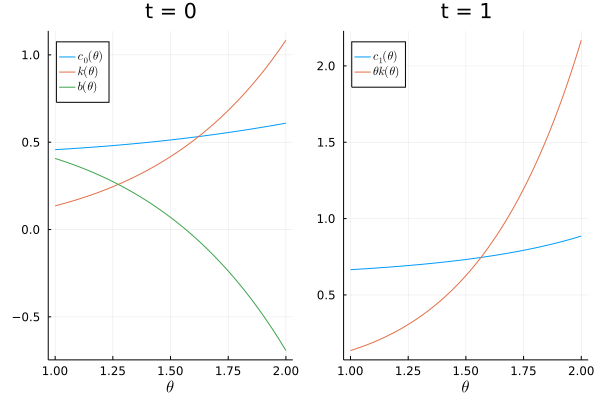
\includegraphics[width = 0.7\textwidth]{figures/allocations.png}
    \label{fig:static_allocs}
\end{figure}

Figure \ref{fig:static_wedges} shows the wedges in the static model, which confirm the analytic results in section \ref{subsec:analytic}. Both wedges are positive and, as demonstrated in Lemma \ref{lem:tauk_bigger}, \( \tau_k>\tau_b \) across the entirety of \( \Theta \), with the exception of \( \underline{\theta} \) and \( \overline{\theta} \). Both wedges are indeed increasing over at least a portion of \( \Theta \). As demonstrated in \eqref{eq:tauk_tpr} and \eqref{eq:taub_tpr}, the wedges are driven by similar forces, and so their shapes are determined by their relative sensitivities to these forces. As anticipated in section \ref{subsec:analytic}, the wedges are increasing in \( \theta \) beyond the point \( \theta^* \) where the ratio \( \theta p\left( \theta \right)/R \) attains its maximum, denoted in Figure \ref{fig:static_wedges} by the vertical black line. Figure \ref{fig:determs} shows the two determinants of the wedges in \eqref{eq:tauk_tpr} and \eqref{eq:taub_tpr}, \( k/c_0 \) and \( \theta p(\theta) / R \). Clearly, the investment ratio \( k/c_0 \) is increasing, and in fact convex, in \( \theta \). \( \theta p(\theta) / R \), meanwhile, is hump-shaped, as suggested by Lemma \ref{lem:thetap}. So, at higher values of \( \theta \), the two forces shown in Figure \ref{fig:determs} pull the wedges in opposite directions. The slope of \( k/c_0 \) in \( \theta \) is increasing, which pulls the wedges up. The slope of \( \theta p/R \) above \( \theta^* \), meanwhile, is decreasing, and more so near \( \overline{\theta} \) as informational rents decrease. The slope of the wedges, then, depends on which of these forces dominates. We can also see from Figure \ref{fig:static_wedges} that \( \tau_k \) and \( \tau_b \) attain their maxima at different values of \( \theta \). In particular, the wedge on savings \( \tau_b \) is progressive over a large range of types, suggesting that this wedge is less sensitive to the downward pull of \( \theta p / R \), as compared to the wedge on investment.

\begin{figure}[htbp]
    \centering
    \caption{Wedges in the Static Model}
    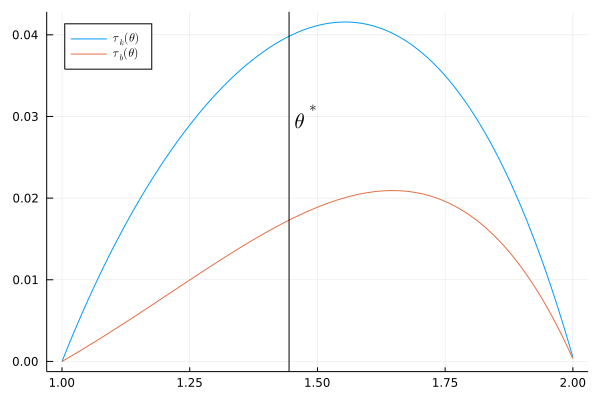
\includegraphics[width = 0.7\textwidth]{figures/wedges.png}
    \label{fig:static_wedges}
    \caption*{\textit{Note: \( \theta^* \) denotes the value of \( \theta \) where the ratio \( \frac{\theta p\left( \theta \right)}{R} \) attains its maximum and begins to decline. This ratio is the force that ultimately pulls the wedges down.}}
\end{figure}

\begin{figure}[htbp]
    \centering
    \caption{Determinants of Wedges in the Static Model}
    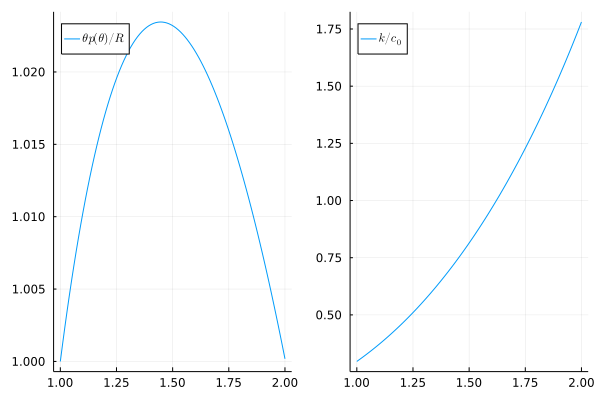
\includegraphics[width = 0.7\textwidth]{figures/determs.png}
    \label{fig:determs}
\end{figure}

\section{Dynamic Model} \label{sec:dyn_mod}

\subsection{IID Case}

In the dynamic setting time is discrete, and agents draw a type $\theta_{t}$
in each period. We assume that these draws are i.i.d.; that is, $\theta_{t}\sim F(\theta)$
for all $t$. Let $\theta^{t}=\left\{ \theta_{0},\theta_{1},...,\theta_{t}\right\} $
denote the history of shocks up to time $t$. Each period plays out
as follows: an agent begins the period by realizing his capital income
\begin{equation}
    y_{t}\left(\theta^{t-1}\right)=p_{t}\left(\theta^{t-1}\right)\theta_{t-1}k_{t}\left(\theta^{t-1}\right) \label{eq:dyn_yt}
\end{equation}
according to prior type $\theta_{t-1}$ and investment $k_{t}$ (made
at time $t-1$), taking as given $p_{t}\left(\theta^{t-1}\right)$.
Then, the agent draws type $\theta_{t}$ from $F$, and makes consumption
and savings choices $\left\{ c_{t}\left(\theta^{t}\right),k_{t+1}\left(\theta^{t}\right),b_{t+1}\left(\theta^{t}\right)\right\} $.
Let $\mu_{t}\left(\theta^{t}\right)$ be the measure of period-$t$
histories induced by the stochastic process for $\theta_{t}$. 

On the production side, the aggregate producer creates final goods
according to a two-step process. First, she combines the intermediate
goods produced by the entrepreneurs into a single capital good $K_{t,f}$
using a CES aggregator, as in the static model\footnote{We use the \( f \) subscript to differentiate the capital used in production from aggregate capital in the economy, \( \int k_{t+1}\left( \theta^t \right)d\mu_t \). \cite{guvenen2019use} refer to the former as the ``quality-adjusted capital stock.''}. She then combines
this capital good with fixed labor quantity $L$ to produce the final
good using a Cobb-Douglas production function\footnote{We include labor, which is in fixed supply, to ensure that the economy does not grow without bound.}. Thus, her production
function has the form 
\begin{equation}
Y_{t}=K_{t,f}^{\alpha}L^{1-\alpha}
\end{equation}
where 
\begin{equation}
K_{t,f}=\left(\int\left[\theta_{t-1}k_{t}\left(\theta^{t-1}\right)\right]^{\frac{\varepsilon-1}{\varepsilon}}d\mu_{t-1}\left(\theta^{t-1}\right)\right)^{\frac{\varepsilon}{\varepsilon-1}} \label{eq:dyn_ktf}
\end{equation}
Thus, the final good producer solves 
\begin{equation}
\max_{y\left(\theta\right)}\ \left[\left(\int\left[\theta_{t-1}k_{t}\left(\theta^{t-1}\right)\right]^{\frac{\varepsilon-1}{\varepsilon}}d\mu_{t-1}\left(\theta^{t-1}\right)\right)^{\frac{\varepsilon}{\varepsilon-1}}\right]^{\alpha}L^{1-\alpha}-\int p_{t}\left(\theta^{t-1}\right)y_{t}\left(\theta\right)d\mu_{t-1}\left(\theta^{t-1}\right)
\end{equation}
and so the price that an entrepreneur of type \( \theta^t \) is paid for his intermediate good variety is 
\begin{equation}
p_{t}\left(\theta^{t-1}\right)=\alpha\left(\frac{L}{K_{t,f}}\right)^{1-\alpha}\left(\frac{K_{t,f}}{\theta_{t-1}k_{t}\left(\theta^{t-1}\right)}\right)^{\frac{1}{\varepsilon}} \label{eq:dyn_pt}
\end{equation}
Note that although aggregate capital exhibits constant returns to
scale, we now have a fixed factor of production (labor), so we will
have a steady state at least in aggregates. From here on, we will normalize \( L \) to one, and thus assume that \( Y_t = K_{t,f}^\alpha \), where \( K_{t,f} \) is defined in \eqref{eq:dyn_ktf}. 

In the dynamic setting, the social planner chooses allocations $\left\{ c_{t}\left(\theta^{t}\right),k_{t+1}\left(\theta^{t}\right)\right\} _{t=0}^{\infty}$
to solve 
\begin{equation}
\max\sum_{t=0}^{\infty}\beta^{t}\int u\left(c_{t}\left(\theta^{t}\right)\right)d\mu_{t}\left(\theta^{t}\right)\label{eq:dyn_plan}
\end{equation}
Subject to feasibility: 
\begin{equation}
\int\left[c_{t}\left(\theta^{t}\right)+k_{t+1}\left(\theta^{t}\right)\right]d\mu_{t}\left(\theta^{t}\right)=\left(\int\left[\theta_{t-1}k_{t}\left(\theta^{t-1}\right)\right]^{\frac{\varepsilon-1}{\varepsilon}}d\mu_{t-1}\left(\theta^{t-1}\right)\right)^{\frac{\alpha\varepsilon}{\varepsilon-1}}\label{eq:dyn_feas1}
\end{equation}
Note that with $p_{t}\left(\theta^{t-1}\right)$ defined as in \eqref{eq:dyn_pt},
we can rewrite the above feasibility constraint as 
\begin{equation}
\int\left[c_{t}\left(\theta^{t}\right)+k_{t+1}\left(\theta^{t}\right)\right]d\mu_{t}\left(\theta^{t}\right)=\int\theta_{t-1}p_{t}\left(\theta^{t-1}\right)k_{t}\left(\theta^{t-1}\right)d\mu_{t-1}\left(\theta^{t}\right)\label{eq:dyn_feas2}
\end{equation}
Promise utility allocated to an agent of history $\theta^{t}$ is
\begin{equation}
w_{t+1}\left(\theta^{t}\right)=\sum_{s=t+1}^{\infty}\beta^{s-t-1}\int u\left(c_{s}\left(\theta^{s}\right)\right)d\mu_{s}\left(\theta^{s}\big|\theta^{t}\right)
\end{equation}
Thus the incentive constraint is 
\begin{multline}
u\left(c_{t}\left(\theta^{t}\right)\right)+\beta w_{t+1}\left(\theta^{t}\right)\ge u\left(c_{t}\left(\left\{ \theta^{t-1},\hat{\theta}_{t}\right\} \right)+k_{t+1}\left(\left\{ \theta^{t-1},\hat{\theta}_{t}\right\} \right)-\frac{\hat{\theta}_{t}k\left(\left\{ \theta^{t-1},\hat{\theta}_{t}\right\} \right)}{\theta_{t}}\right)+\\
\beta w_{t+1}\left(\left\{ \theta^{t-1},\hat{\theta}_{t}\right\} \right)
\end{multline}
and, following from the static environment, the local incentive constraint is: 
\begin{equation}
U^{\prime}\left(\theta^{t}\right)=u^{\prime}\left(c_{t}\left(\theta^{t}\right)\right)\frac{k_{t+1}\left(\theta^{t}\right)}{\theta_{t}}\label{eq:dyn_ic}
\end{equation}

We focus on the dual to the planner's problem in \eqref{eq:dyn_plan}, wherein the planner minimizes the cost of providing allocations to achieve a prespecified level of lifetime utility \( U^* \). Using the definition of feasibility in \eqref{eq:dyn_feas2}, the cost minimization problem is 
\begin{equation}
    \min\sum_{t=0}^{\infty}\left(\prod_{s=0}^{t-1}R_{s}\right)^{-1}\left\{ \int\left[c_{t}\left(\theta^{t}\right)+k_{t+1}\left(\theta^{t}\right)\right]d\mu_{t}\left(\theta^{t}\right)-\int p_{t}\left(\theta^{t-1}\right)\theta_{t-1}k_{t}\left(\theta^{t-1}\right)d\mu_{t-1}\left(\theta^{t-1}\right)\right\} \label{eq:cost_obj}
\end{equation}
subject to 
\begin{equation}
    \sum_{t=0}^{\infty}\beta^{t}\int u\left[c_{t}\left(\theta^{t}\right)\right]d\mu_{t}\left(\theta^{t}\right)\ge U^{*}\label{eq:cost_constr}
\end{equation}
along with the local incentive constraints in (\ref{eq:dyn_ic}).

\subsection{Solving the Planning Problem}
We can define aggregate consumption and investment as follows: 
\begin{align}
    C_{t}&=\int c_{t}\left(\theta^{t}\right)d\mu_{t}\left(\theta_{t}\right)\\
    K_{t+1}&=\int k_{t+1}\left(\theta^{t}\right)d\mu_{t}\left(\theta_{t}\right)
\end{align}
If a steady state exists, then these values, along with \( K_{t,f} \) and \( Y_t \), will be constant. We can thus denote the steady-state aggregates as \( C^*,K^*,K_f^*,Y^* \). 

The next step to solving is to notice that the planner's problem in \eqref{eq:cost_obj} is homogeneous in \( U^* \). As such, we can write the policy function for \( k_{t+1}\left( \theta^t \right) \) as 
\begin{align*}
    k_{t+1}\left(\theta^{t}\right)&=\overline{k}_{t+1}\left(\theta_{t}\right)\exp\left[\left(1-\beta\right)w_{t}\left(\theta^{t-1}\right)\right]\\&=\overline{k}_{t+1}\left(\theta_{t}\right)\exp\left[\left(1-\beta\right)\left(w^{\prime}\left(\theta_{t-1}\right)+w^{\prime}\left(\theta_{t-2}\right)+...+w^{\prime}\left(\theta_{0}\right)+w_{0}\right)\right]
\end{align*}
Using the above policy function, we can decompose the price earned by an entrepreneur producing variety \( \theta^t \) as follows: 
\begin{align*}
    p_{t+1}\left(\theta^{t}\right)&=\alpha K_{f}^{\alpha-1}K_{f}^{\frac{1}{\varepsilon}}\left(\theta_{t}k_{t+1}\left(\theta^{t}\right)\right)^{-\frac{1}{\varepsilon}}\\&=\alpha K_{f}^{\alpha-1}K_{f}^{\frac{1}{\varepsilon}}\left(\theta_{t}\overline{k}_{t+1}\left(\theta_{t}\right)\exp\left[\left(1-\beta\right)w_{t}\left(\theta^{t-1}\right)\right]\right)^{-\frac{1}{\varepsilon}}\\&=\underbrace{\alpha K_{f}^{\alpha-1}K_{f}^{\frac{1}{\varepsilon}}\exp\left[-\frac{\left(1-\beta\right)}{\varepsilon}\left(w^{\prime}\left(\theta_{t-1}\right)+w^{\prime}\left(\theta_{t-2}\right)+...+w^{\prime}\left(\theta_{0}\right)+w_{0}\right)\right]^{-\frac{1}{\varepsilon}}}_{\overline{p}_{t}\left(\theta^{t-1}\right)}\underbrace{\left(\theta_{t}\overline{k}_{t+1}\left(\theta_{t}\right)\right)^{-\frac{1}{\varepsilon}}}_{\hat{p}_{t}\left(\theta_{t}\right)}
\end{align*}
The final line shows our desired result: because of the homogeneity of this problem, we can decompose the price \( p_{t+1}\left(\theta^{t}\right) \) into two components \( \overline{p}_{t}\left(\theta^{t-1}\right) \), which depends on the history \( \theta^{t-1} \), and \( \hat{p}_t\left( \theta_t \right) \), which depends only on current type. Because \( \overline{p}_{t}\left(\theta^{t-1}\right) \) is common among all agents with prior history \( \theta^{t-1} \)--equivalently, those with promised utility \( w_t\left( \theta^{t-1} \right) \)--we refer to \( \bar{p}_t \) as the ``common price.'' Advancing forward one period in time, we can see that \( \bar{p}_{t+1} \) is given by 
\begin{align*}
    \overline{p}_{t+1}\left(\theta^{t}\right)&=Y^{\frac{1}{\varepsilon}}\exp\left[\left(1-\beta\right)\left(w^{\prime}\left(\theta_{t}\right)+w^{\prime}\left(\theta_{t-1}\right)+...+w^{\prime}\left(\theta_{0}\right)+w_{0}\right)\right]^{-\frac{1}{\varepsilon}}\\&=\overline{p}_{t}\left(\theta^{t-1}\right)\underbrace{\exp\left[-\frac{\left(1-\beta\right)}{\varepsilon}w^{\prime}\left(\theta_{t}\right)\right]}_{\tilde{p}\left(\theta_{t}\right)}
\end{align*}
Thus, the common price evolves according to 
\begin{equation}
    \overline{p}_{t+1}\left(\theta^{t}\right)=\overline{p}_{t}\left(\theta^{t-1}\right)\tilde{p}\left(\theta_{t}\right) \label{eq:pbar_next}
\end{equation}
and the total price earned will be given by 
\begin{equation}
    p_{t+1}\left(\theta^{t}\right)=\overline{p}_{t}\left(\theta^{t-1}\right)\hat{p}_{t}\left(\theta^{t}\right) \label{eq:price_decomp}
\end{equation}
\subsubsection{Recursive Formulation}
In order to simplify our analysis, we focus our attention on the problem of a \textit{component planner}, who solves the cost minimization problem in \eqref{eq:cost_obj} for an agent with a particular history \( \theta^t \), assuming that interest rates are constant over time. There are two state variables in the component planner's problem: promise utility \( w \) and common price \( \bar{p} \). Because the productivity shocks are IID, promise utility \( w \) is a sufficient statistic for the history of shocks \( \theta^t \). The common price \( \bar{p} \), meanwhile, is needed to determine the return that the agent will earn on today's investment, using the formula in \eqref{eq:price_decomp}. In general equilibrium, we can see from \eqref{eq:pbar_next} that all agents of history \( w \) will have a common \( \bar{p} \). However, because the households are price-takers, the component planner does not internalize this fact, and thus, she must keep track of \( \bar{p} \). Suppressing the dependence of allocations on \( w \) and \( \bar{p} \), then, the component planner's problem in recursive form is 
\begin{align}
    C(w,\overline{p})=\min_{\substack{c(\theta),k^{\prime}(\theta),\\
w^{\prime}(\theta),U(\theta) \label{eq:dyn_cmp}
}
}&\int\left\{ c\left(\theta\right)+k^{\prime}\left(\theta\right)+\frac{1}{R}\left[C\left(w^{\prime}\left(\theta\right),\overline{p}\cdot\tilde{p}\left(\theta\right)\right)-\overline{p}\cdot\hat{p}\left(\theta\right)\theta k^{\prime}\left(\theta\right)\right]\right\} dF\left(\theta\right)\\
&\text{subject to} \notag \label{eq:dyn_pkc} \\
\int U(\theta)dF(\theta)&\ge w\\
U(\theta)&=u\left(c(\theta)\right)+\beta w^{\prime}(\theta)\\U^{\prime}(\theta)&=u^{\prime}\left(c(\theta)\right)\frac{k^{\prime}(\theta)}{\theta} \label{eq:dyn_lic}
\end{align}
Note that we exploit the decomposition of prices outlined above in order to pose the problem in a way that is homogeneous in \( w \). As such, we have the following proposition: 
\begin{proposition} \label{prop:vf_homog}
    Suppose that \( u(c) = \ln c \). Then, the solution to the planner's problem in \eqref{eq:dyn_cmp}-\eqref{eq:dyn_lic} has the following form:
    \begin{align*}
        C\left(w,\overline{p}\right)&=A\left(\overline{p}\right)e^{\left(1-\beta\right)w}&w^{\prime}\left(\theta,w,\overline{p}\right)&=w^{\prime}\left(\theta,\overline{p}\right)+w\\c\left(\theta,w,\overline{p}\right)&=c\left(\theta,\overline{p}\right)e^{\left(1-\beta\right)w}&U\left(\theta,w,\overline{p}\right)&=U\left(\theta,\overline{p}\right)+w\\k^{\prime}\left(\theta,w,\overline{p}\right)&=k^{\prime}\left(\theta,\overline{p}\right)e^{\left(1-\beta\right)w}&&
    \end{align*}
    for some \( A\left( \overline{p} \right),c(\theta,\overline{p}),k^{\prime}(\theta,\overline{p}),w^{\prime}(\theta,\overline{p}) \), and \( U(\theta,\overline{p}) \).
\end{proposition}

The proof can be found in the Appendix. At the time of writing, we are working on developing a solution to the planner's problem above, which amounts to solving for the ``baseline'' allocations \( A\left( \overline{p} \right),c(\theta,\overline{p}),k^{\prime}(\theta,\overline{p}),w^{\prime}(\theta,\overline{p}) \), and \( U(\theta,\overline{p}) \).

\section{Conclusion} \label{sec:concl}

This paper has studied the optimal taxation of capital income when agents are heterogeneous in the rates of return on their investments. In a static setting, we have demonstrated that the optimality of positive capital income taxation established in \cite{golosov2003optimal} is preserved when agents earn heterogeneous returns, rather than a common rate. We show that in this setting, the wedges on both net-zero savings and investment are hump-shaped, and thus increasing in return over a portion of the type distribution. Furthermore, we demonstrate that the wedges faced by a given type are a function of two forces: the ratio of investment to consumption in the optimal allocations, and the ratio of the societal marginal product of capital for this type to the common rate earned on savings. 

In the dynamic context, we exploit the homogeneity of the planner's value function in order to decompose prices, which allows us to formulate the \textit{component} planner's problem in a way that maintains the homogeneity of the overall problem. Our next step is to solve this recursive formulation, which will allow us to characterize optimal wedges in the dynamic setting. Once we have established results in the IID case, we will turn to the case where returns are persistent, using the techniques from \cite{farhi2013insurance}. Finally, we will attempt to construct a tax and transfer scheme that implements the constrained-efficient allocations in a competitive equilibrium. 

\bibliographystyle{named}
\bibliography{summer_paper}
\newpage
\section*{Appendix}
\setcounter{equation}{0}
\renewcommand{\theequation}{A.\arabic{equation}}

\subsection*{Proof of Lemma \ref{lem:thetap}}
\begin{proof}
    To begin, the first-order conditions for \( c_0(\theta) \) and \( k(\theta) \) respectively in the static problem can be written as follows: 
    \begin{align}
        R&=\frac{c_{1}}{\beta c_{0}}-\frac{k}{\lambda_{1}\theta c_{0}^{2}}\mu \label{eq:foc_c0} \\ 
        R &= \theta p\left(\theta\right)+\frac{\mu}{\lambda_{1}\theta c_{0}} \label{eq:foc_k}
    \end{align}
    The proof is somewhat self-evident. Because it represents the multiplier on an equality constraint, we know that on the interior of \( \Theta \), \( \mu\ne 0 \), which implies from \eqref{eq:foc_k} that \( R \ne \theta p(\theta) \). Suppose that for an agent with type \( \theta \), at the optimum \( R>\theta p \). From the first-order conditions above, this implies that \( \mu>0 \), and \( R<c_1 / (\beta c_0) \).
    
    If this were the case, however, then the agent would be investing to the point where his \textit{societal} marginal product of capital was less than the common rate. Clearly, such a prescription is not optimal: the planner could call for the agent to invest less in his entrepreneurial technology, and save the remainder in the common-rate asset. Such a transfer would create resources, some of which could be used to maintain incentive compatibility. Thus, it must be that wherever the distortions are nonzero, \( R<\theta p(\theta) \). 
\end{proof}

\subsection*{Proof of Lemma \ref{lem:tauk_bigger}}
\begin{proof}
    Using the formulae for the wedges in \eqref{eq:tauk_tpr} and \eqref{eq:taub_tpr}, we can relate the wedges in the following way: 
    \begin{align*}
        \tau_{k}\left(\theta\right)&=\left(1+\tau_{b}\left(\theta\right)\left(\frac{\theta p\left(\theta\right)}{R}-1\right)\right)\underbrace{\left(1-\frac{R}{\theta p\left(\theta\right)}\right)}_{\equiv\kappa\left(\theta\right)}\\&=\kappa\left(\theta\right)+\tau_{b}\left(\theta\right)\left(\frac{\kappa\left(\theta\right)}{1-\kappa\left(\theta\right)}\right)
    \end{align*}
    By lemma \ref{lem:thetap}, \( \kappa(\theta)>0 \) and \( 1-\kappa(\theta)>0 \). Thus, for \( \theta\in\left(\underline{\theta},\overline{\theta}\right) \), \( \tau_{k}>\tau_{b} \). Both distortions are zero for \( \underline{\theta} \) and \( \overline{\theta} \). 
\end{proof}

\subsection*{Proof of Proposition \ref{prop:vf_homog}}
\begin{proof}
    Under the conjectured form, with $w=0$ the Bellman equation becomes
\begin{equation}
A\left(\overline{p}\right)=\min_{\substack{c(\theta),k^{\prime}(\theta),\\
w^{\prime}(\theta),U(\theta)
}
}\int\left[c\left(\theta\right)+k^{\prime}\left(\theta\right)+\frac{1}{R}\left\{ A\left(\overline{p}\cdot\tilde{p}\left(\theta\right)\right)\exp\left(\left(1-\beta\right)w^{\prime}(\theta)\right)-\overline{p}\cdot\hat{p}\left(\theta\right)\theta k^{\prime}\left(\theta\right)\right\} \right]dF\left(\theta\right)\label{eq:logu_aw}
\end{equation}
subject to 
\begin{align}
0 & =\int U(\theta,\overline{p})dF(\theta)\label{eq:logu_pkc}\\
U(\theta,\overline{p}) & =\ln\left(c(\theta,\overline{p})\right)+\beta w^{\prime}(\theta,\overline{p})\\
U^{\prime}(\theta,\overline{p}) & =\frac{k^{\prime}(\theta,\overline{p})}{\theta c(\theta,\overline{p})}\label{eq:logu_lic}
\end{align}
From the component planner's perspective, this problem is now independent
of $w$. Assuming $R>1$, by Blackwell's sufficient conditions the
mapping on the RHS of (\ref{eq:logu_aw}) is a contraction mapping,
with fixed point $A(\cdot)$. Because this fixed point is independent
of $w$, the function $A$ is also independent of $w$. Finally, note
that if the baseline allocations $c\left(\theta\right),k^{\prime}\left(\theta\right),w^{\prime}\left(\theta\right)$,
and $U\left(\theta\right)$ satisfy the constraints (\ref{eq:logu_pkc})-(\ref{eq:logu_lic})
of the problem when $w=0$. Then, given any $w$, the conjectured
policy functions will also satisfy (\ref{eq:logu_pkc})-(\ref{eq:logu_lic}):
\begin{align}
\int U(\theta,w,\overline{p})dF(\theta) & =\int\left[U(\theta,\overline{p})+w\right]dF(\theta)\label{eq:polfun_proof_1}\\
 & =\int U(\theta,\overline{p})dF(\theta)+w\nonumber \\
\ln\left(c(\theta,w,\overline{p})\right)+\beta w^{\prime}(\theta,w,\overline{p}) & =\ln\left[c\left(\theta,\overline{p}\right)e^{\left(1-\beta\right)w}\right]+\beta\left(w^{\prime}\left(\theta,\overline{p}\right)+w\right)\\
 & =\ln c(\theta,\overline{p})+\beta w^{\prime}\left(\theta,\overline{p}\right)\nonumber \\
\frac{\partial}{\partial\theta}U\left(\theta,w,\overline{p}\right) & =\frac{k^{\prime}\left(\theta,w,\overline{p}\right)}{\theta c\left(\theta,w,\overline{p}\right)}\label{eq:eq:polfun_proof_2}\\
 & =\frac{k^{\prime}(\theta,\overline{p})}{\theta c(\theta,\overline{p})}=U^{\prime}(\theta,\overline{p})\nonumber 
\end{align}
\end{proof}
\end{document}